%%%%%%%%%%%%%%%%%%
% Chapitre 1 - Les engrenages %
%%%%%%%%%%%%%%%%%%

\chapter{Les engrenages}

\section{Introduction}
les engrenages sont des méchanismes utilisés pour transmettre un mouvement ou une puissance entre deux arbres et sont fait en acier, fonte ou matériaux plastiques. ils sont surtout utilisés pour jouer sur les vitesses de rotation : on les réduit ou on les multiplie (plus rare). Elles sont réalisées à l'aide d'une fraiseuse et non par coulage de fer en raison de la géométrie de la pièce et de la précision nécessaire. La théorie qui sera présentée permet une facilité de fabrication et une bonne durée de vie.
	
\section{Historique}
\subsection{Premières tentatives}
\begin{wrapfigure}[4]{l}{3.2cm}
	\vspace{-5mm}
	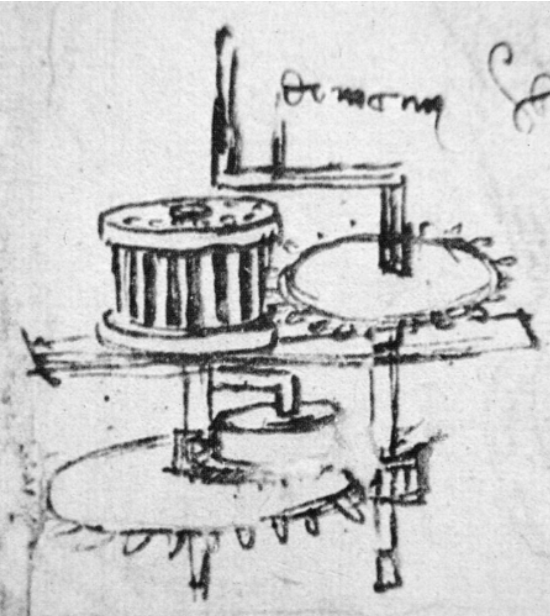
\includegraphics[scale=0.32]{ch1/1}
\end{wrapfigure}
\noindent Les premiers dessins effectués par Léonard de Vinci (15\up{ème} siècle n'étaient pas très clairs, mais on peut apercevoir, sur la figure de gauche, des dentures qui ressemble à celles utilisées aujourd'hui. \\\\\\\\\\\
	
\begin{wrapfigure}[10]{r}{4.6cm}
	\vspace{-5mm}
	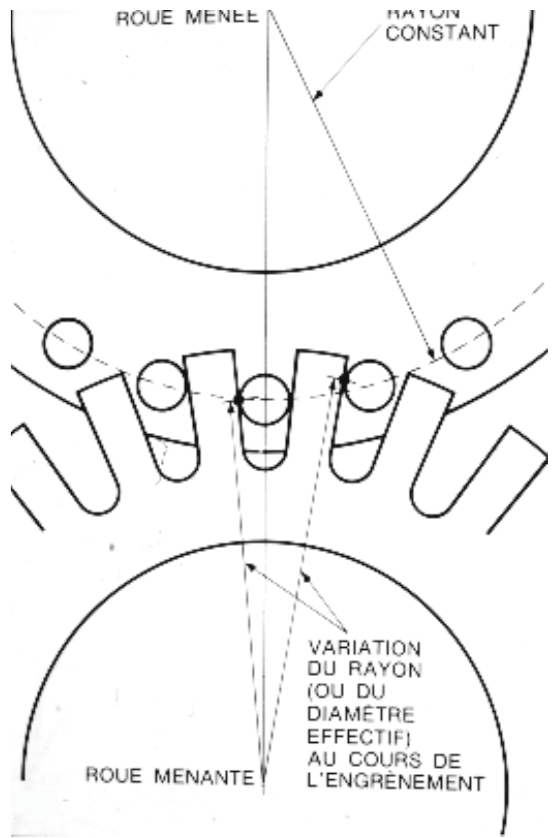
\includegraphics[scale=0.35]{ch1/2}
\end{wrapfigure}	
\noindent Un zoom sur ces fameux modèles permet d'avoir une vue plus moderne. Le problème de ce principe est que la transmission ne se fait pas de manière \textbf{homocinétique} (vitesse de sortie pas constante). La cause est que le point de contact entre la roue menée et la roue menante ne se trouve pas à la même distance (rayon d'entraînement) du centre de la roue menante durant la rotation.  \\
Un second problème est le glissement important qui dégrade le matériel assez rapidement. Ce modèle n'est donc satisfaisant que pour de faibles vitesses et des puissances peu importantes. \\\\
	
\begin{wrapfigure}[4]{l}{4.7cm}
	\vspace{-5mm}
	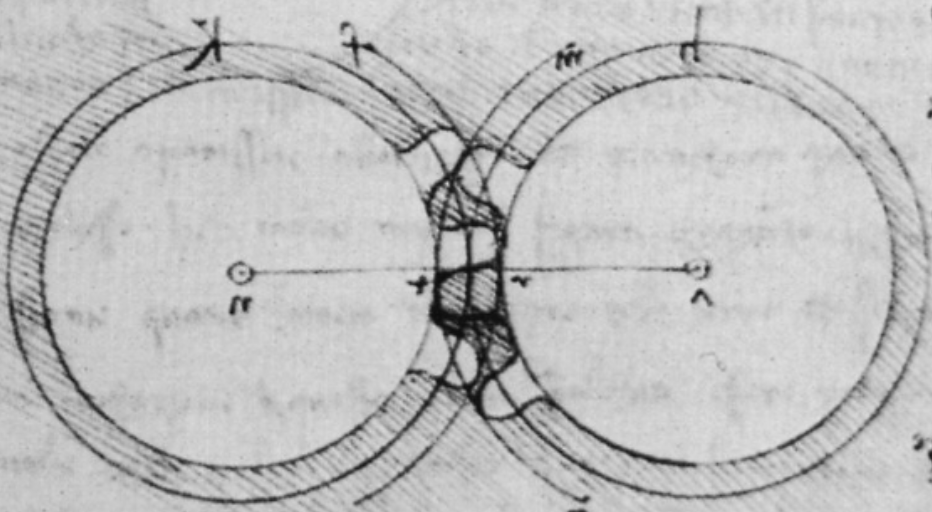
\includegraphics[scale=0.28]{ch1/3}
\end{wrapfigure}	
\noindent Ce dessin de de Vinci témoigne qu'on a cherché à créer une denture qui permettrait de limiter au mieux les deux problèmes majeurs énoncés. \\\\
	
\subsection{La développante de cercle}
\label{subsec:1.2.2}
\begin{wrapfigure}[9]{r}{4cm}
	\vspace{-5mm}
	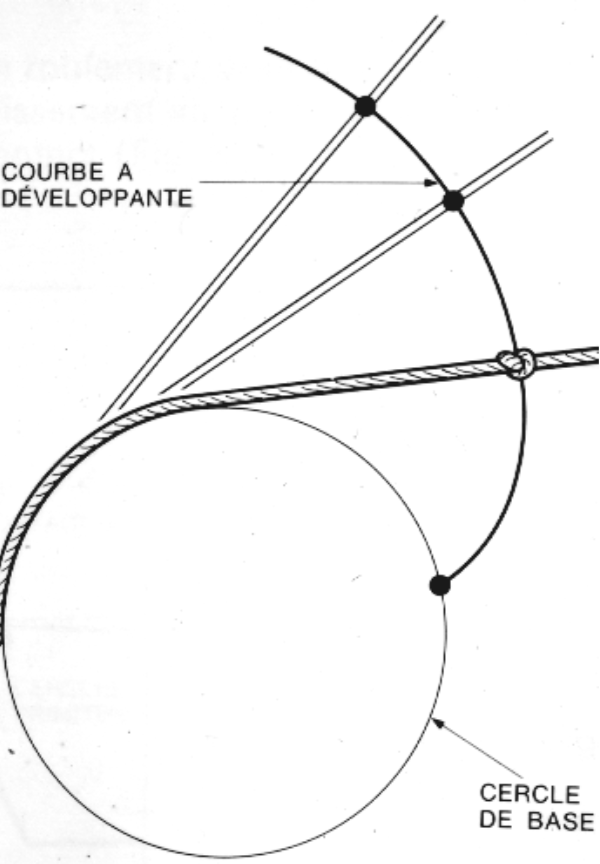
\includegraphics[scale=0.3]{ch1/4}
\end{wrapfigure}	
\noindent La solution adoptée par de Vinci a été de confectionner des dentures en \textbf{développante de cercle}. Il s'agit de la courbe obtenue lorsqu'on "déballe" un fil attaché par une extrémité à un cercle et préalablement accolé à celui-ci. Parmi d'autres théories, celle-ci à l'avantage de pouvoir être mise facilement sous équation et est donc programmable. En plus d'être facile, simple et bon marché, elle permet une \textbf{normalisation facile} afin qu'on ne doive pas faire fabriquer d'engrenages spécifiques. 
	
\section{Généralités}
\begin{wrapfigure}[8]{l}{5.6cm}
	\vspace{-5mm}
	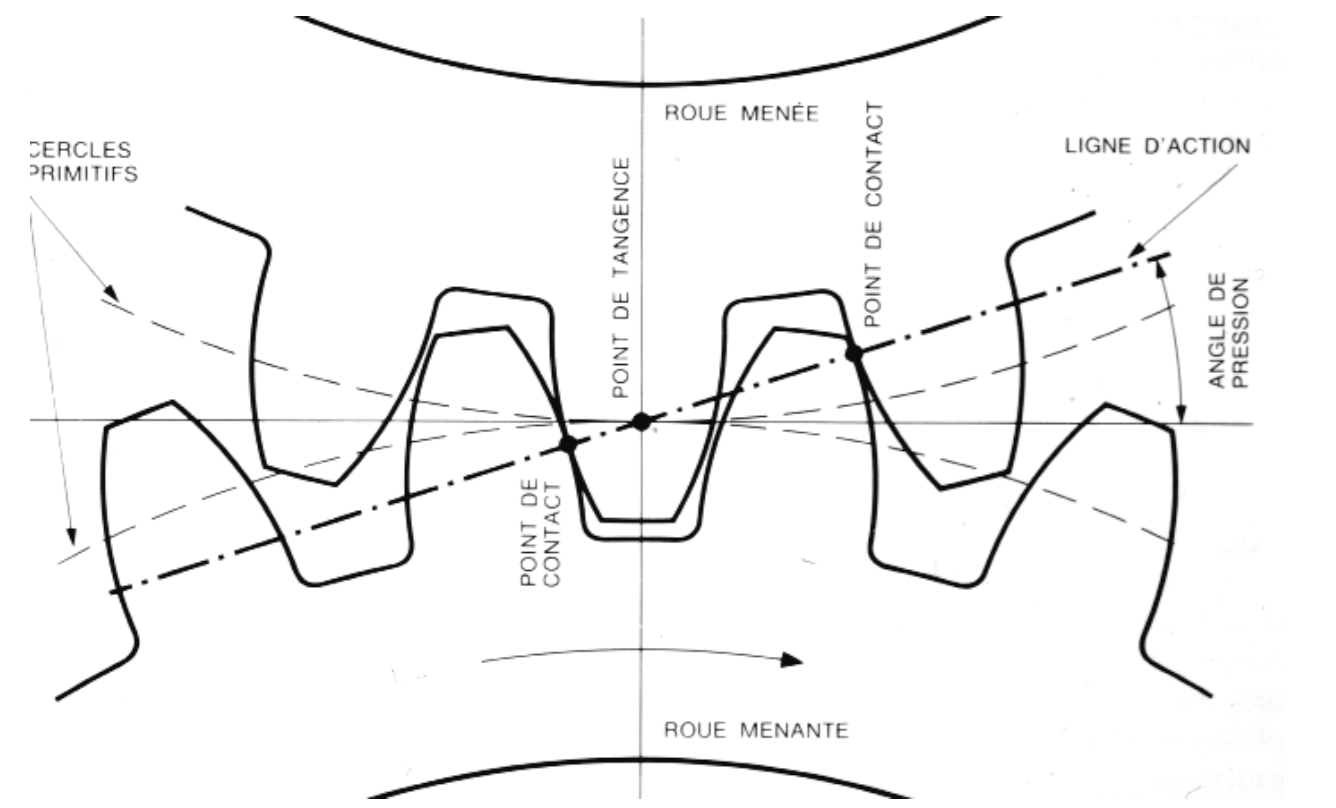
\includegraphics[scale=0.25]{ch1/5}
\end{wrapfigure}	
\noindent Une vue plus complexe nous permet, premièrement, de remarquer que dès le contact de deux nouvelles dents, deux autres rompent leur contact. Deuxièmement, il est possible de tracer deux cercles non tangents sauf en un seul point situé sur normale qui est le \textbf{point de tangence}. Dernièrement, l'évolution du point de contact en fonction du temps décrit une droite, la \textbf{ligne d'action} qui est toujours normale à la surface des dents au point de contact. La force de contact est donc toujours normale à cette surface également. La pente de cette droite est l'\textbf{angle de pression}. Pour transmettre une plus grande force, on a tendance à prendre un grand-angle de pression. \\
	
\begin{wrapfigure}[5]{r}{5.6cm}
	\vspace{-5mm}
	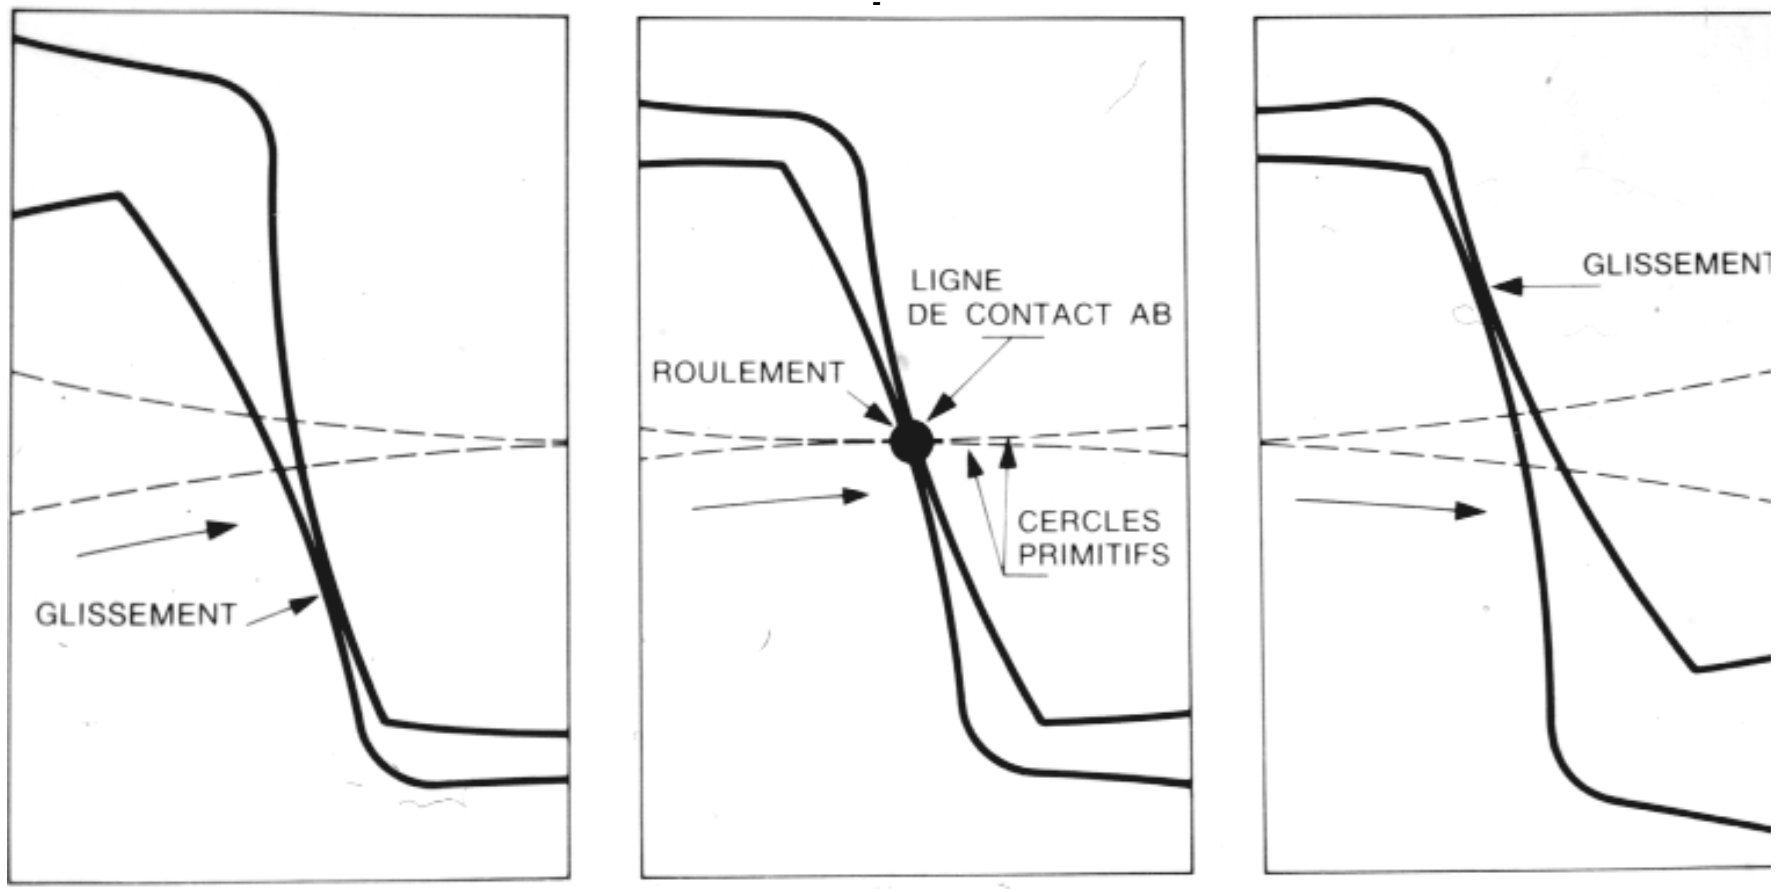
\includegraphics[scale=0.2]{ch1/6}
\end{wrapfigure}	
\noindent Néanmoins, on ne sait pas éviter les glissements. L'\textbf{engrènement} se déroule en 3 phases : une phase de glissement suivie du roulement au niveau du point de contact et une fin avec un nouveau glissement. 

\section{Différents types}
\subsection{Engrenages cylindriques à denture droite}
\begin{wrapfigure}[5]{l}{2.5cm}
	\vspace{-5mm}
	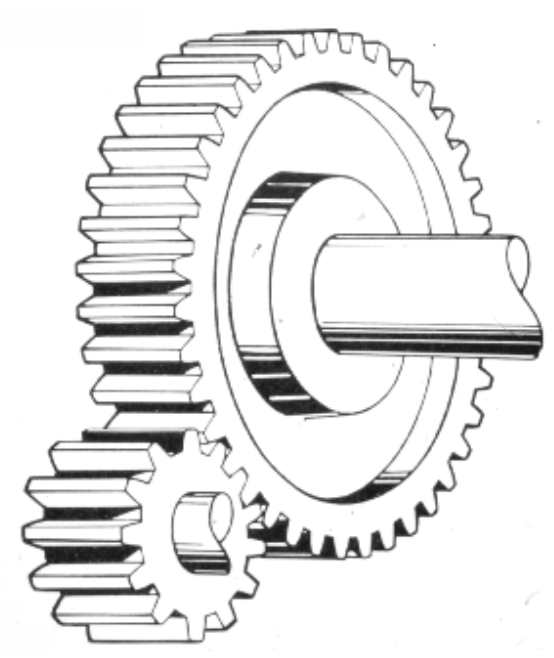
\includegraphics[scale=0.23]{ch1/7}
\end{wrapfigure}	
\noindent Ce modèle d'engrenage est de loin le plus courant. \textbf{Cylindrique} car l'engrenage possède une épaisseur, donnant une longueur aux dents. \textbf{A denture droite} car les dents sont disposées sur les génératrices de ce cylindre. Nous ne nous sommes pas attardés sur les principaux éléments de définition mais citons que l'angle de pression est de $20\degres$. \\
	
\begin{wrapfigure}[5]{r}{2.5cm}
	\vspace{-5mm}
	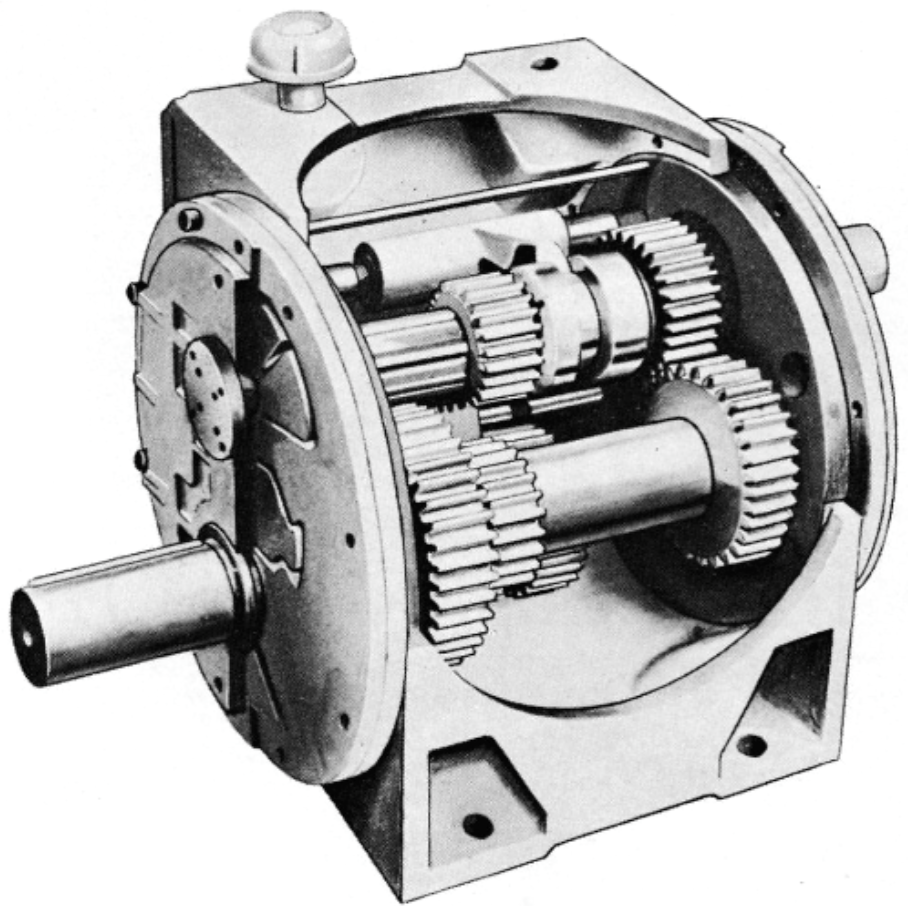
\includegraphics[scale=0.21]{ch1/8}
\end{wrapfigure}	
\noindent On peut bien sûr faire des combinaisons et former des boites d'engrenages. Cependant, ce type d'engrenage, dû à la largeur de la dent, présente l'inconvénient de faire durer le contact assez longtemps. Ceci provoque une flexion des dents et provoque du bruit.
	
\subsection{Contact et sens de rotation}
\begin{itemize}
	\item[$\bullet$] Contact extérieur : sens inverse.
	\item[$\bullet$] Contact intérieur : même sens.
	\item[$\bullet$] Pignon crémaillère : transformation de rotation en translation ou inversément. 
\end{itemize}
	
\subsection{Engrenages cylindriques à denture helicoïdale}
\begin{wrapfigure}[5]{l}{2cm}
	\vspace{-5mm}
	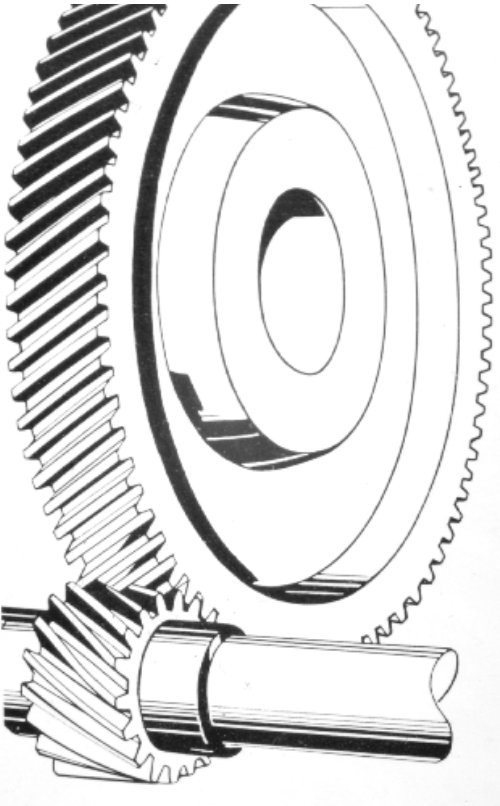
\includegraphics[scale=0.21]{ch1/9}
\end{wrapfigure}	
\noindent Pour remédier au problème de flexion, on réalise un engrènement progressif. Cependant, le problème des efforts radiaux laisse maintenant place aux efforts axiaux qui sont à l'origine de fatigue et d'usure sur les palier de guidage des arbres. Ce modèle est un peu plus compliqué mécaniquement. \\
	
\subsection{Engrenages cylindriques à chevrons}
\begin{wrapfigure}[4]{r}{4cm}
	\vspace{-5mm}
	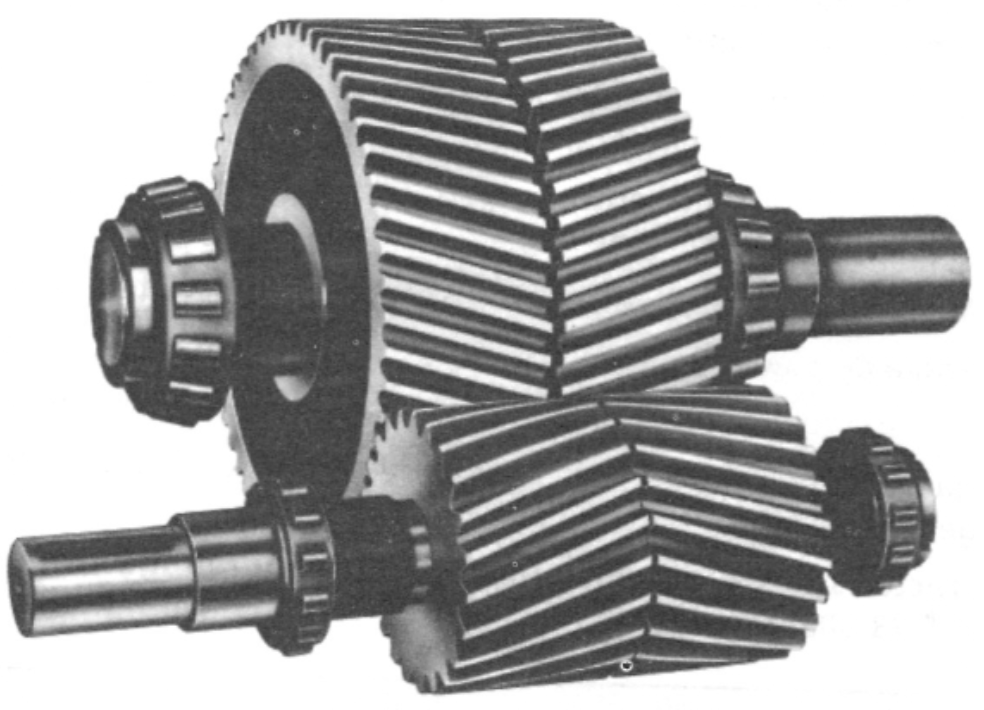
\includegraphics[scale=0.2]{ch1/10}
\end{wrapfigure}	
\noindent En utilisant des roues à chevrons, on espère, par effet opposé, d'annuler les contraintes axiales. Cependant, le coût de fabrication est élevé. \\
	
\subsection{Engrenages coniques}
\begin{wrapfigure}[6]{l}{6.5cm}
	\vspace{-5mm}
	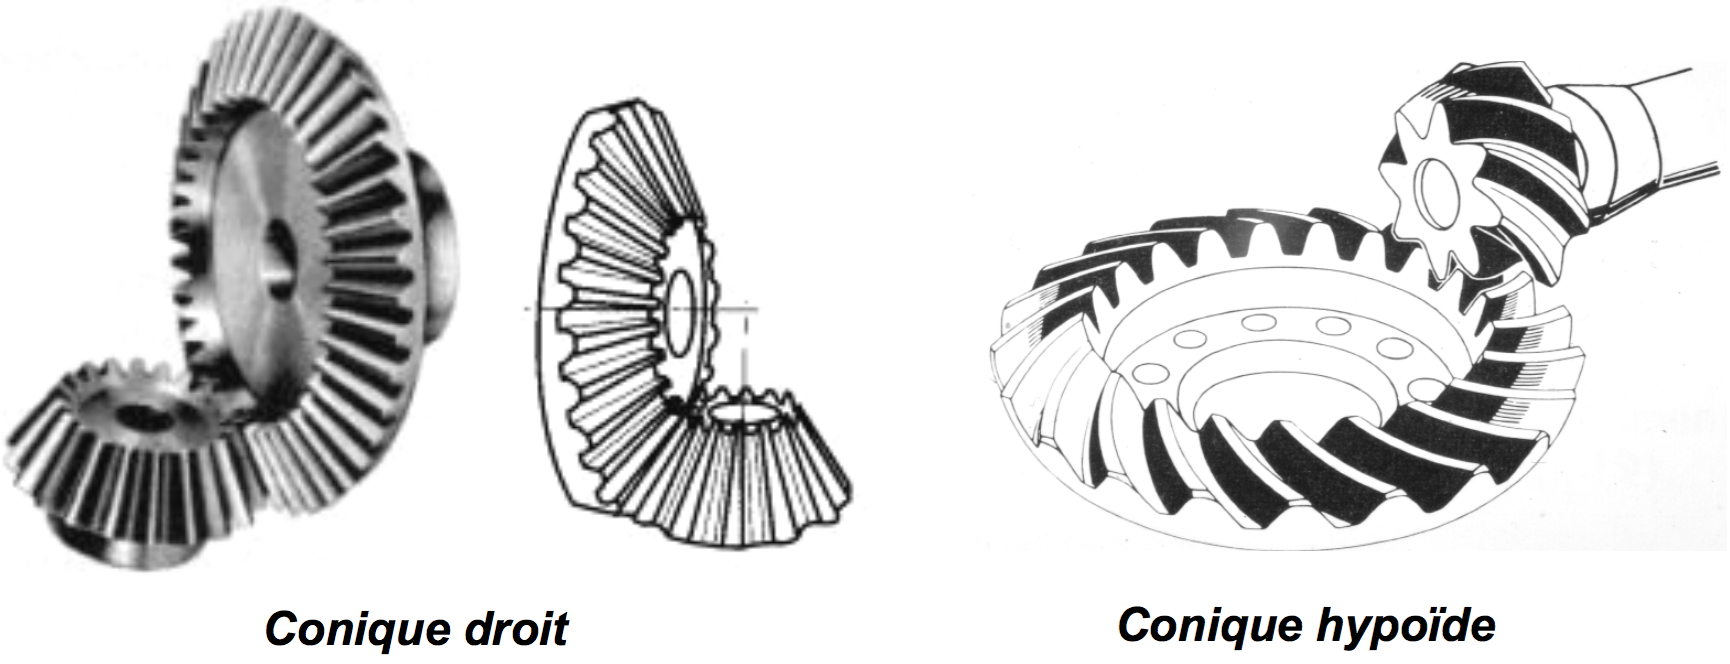
\includegraphics[scale=0.21]{ch1/11}
\end{wrapfigure}	
\noindent Ceux-ci sont utilisés lorsque les axes des engrenages ne sont pas parallèles. On distingue les \textbf{coniques droits} qui sont comparables aux dentures droites et les \textbf{hypoïdes} qui sont en fait les coniques hellicoïdales sauf que la développante de cercle est remplacée par une hypoïde.
	
\subsection{Engrenages gauches hellicoïdaux}
\begin{wrapfigure}[2]{r}{4cm}
	\vspace{-5mm}
	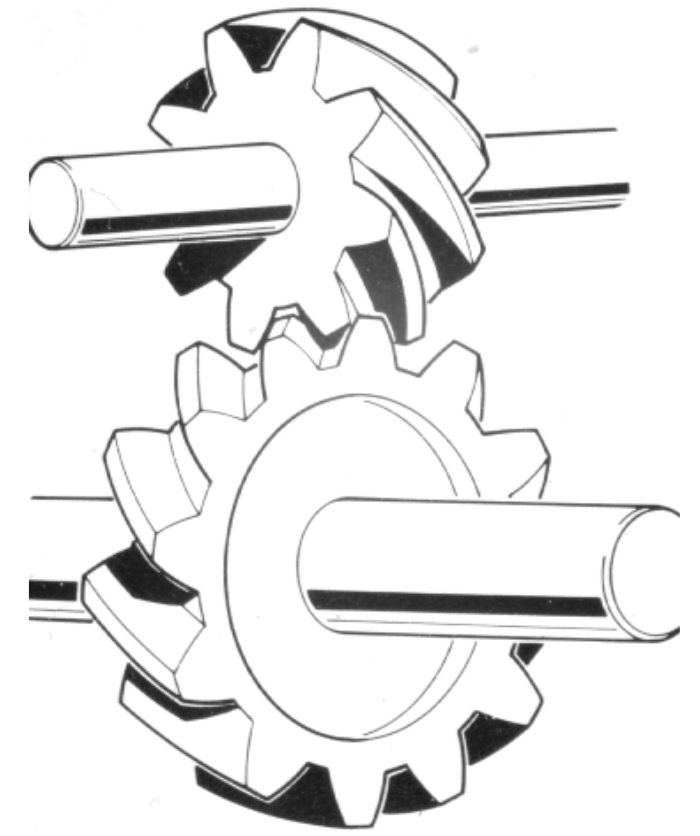
\includegraphics[scale=0.21]{ch1/12}
\end{wrapfigure}	
\noindent Là c'est l'extrême. Utilisé pour des axes quelconque. Très peu utilisé. \\\\\\\\

\subsection{Engrenages à roue et vis sans fin}
\begin{wrapfigure}[6]{l}{2.5cm}
	\vspace{-5mm}
	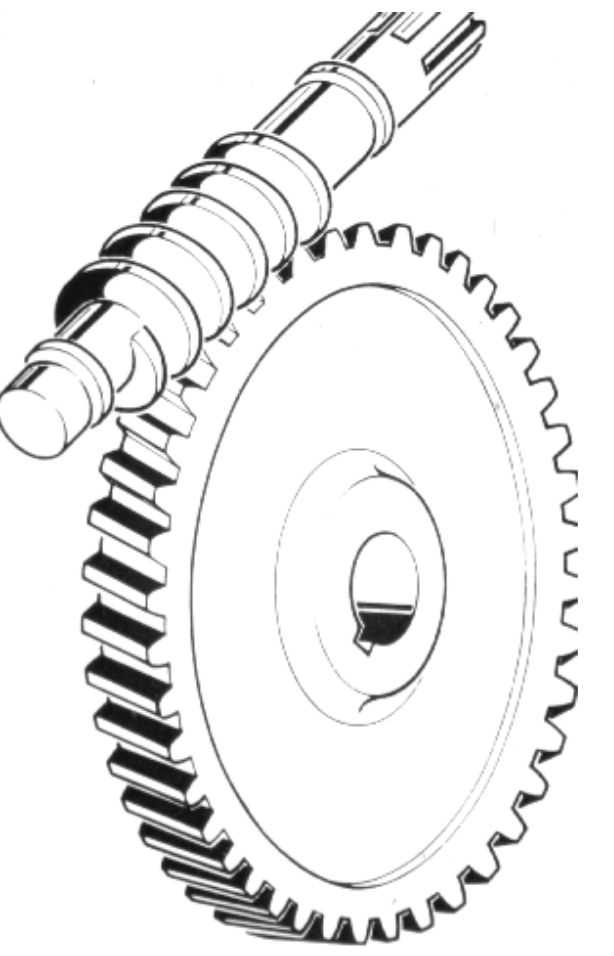
\includegraphics[scale=0.21]{ch1/13}
\end{wrapfigure}	
\noindent Ca ressemble à un pignon crémaillère en 3D qui ne translate pas, mais tourne. Il est intéressants pour le grand rapport de réduction ($\approx 1/200$). Cependant, le rendement est très faible et les glissements sont importants, causant de l'usure. Pour remédier à ce problème de glissement on peut utiliser une \textbf{roue creuse} (même modèle mais creusé. Pour concentrer l'usure sur la roue qui coûte moins cher, la vis est en acier et la roue en bronze (vis peut avoir plusieurs filets). \\
	
\section{Lubrification}
\noindent Pour une bonne lubrfication, il faut créer un \textbf{coin d'huile} qui permette de former une couche épaisse sous le solide en mouvement. Le gradient de pression permettra un meilleur glissement. La forme des dentures et le glissement au début du contact favorise la formation de ce coin d'huile. 

\subsection{Lubrification par barbotage}
\begin{wrapfigure}[5]{r}{4cm}
	\vspace{-5mm}
	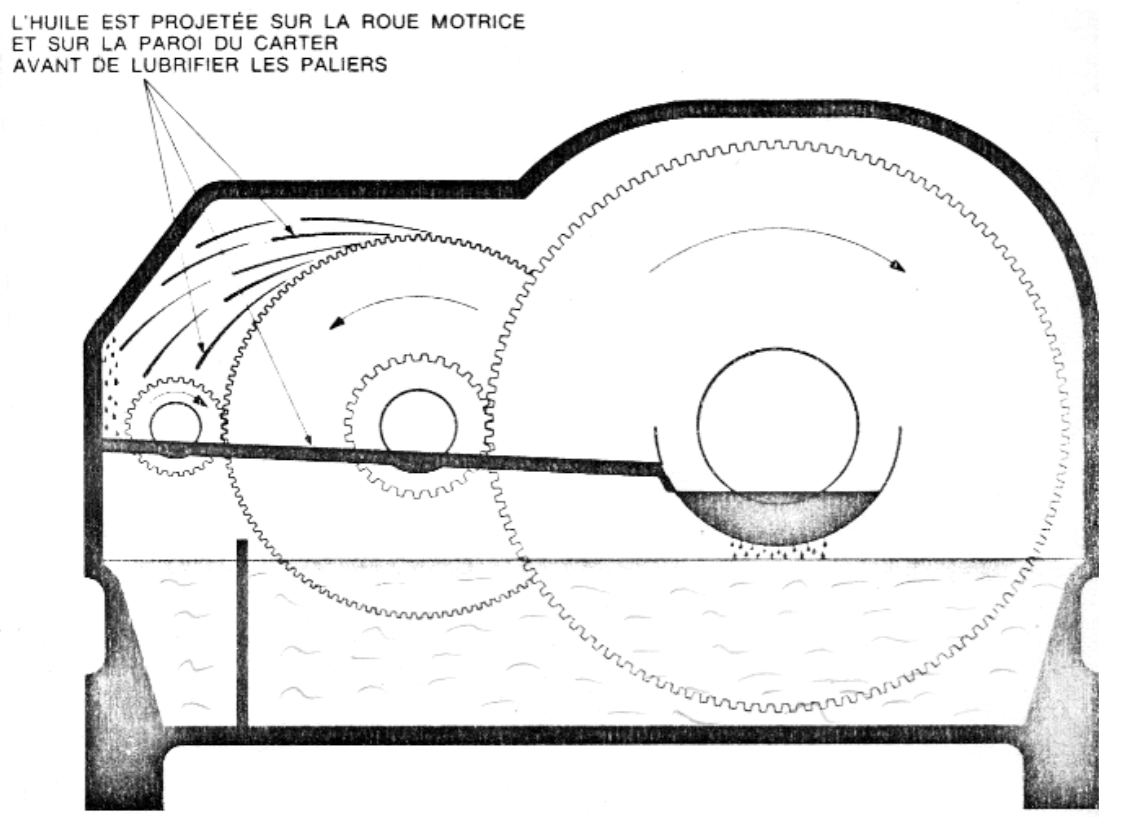
\includegraphics[scale=0.21]{ch1/14}
\end{wrapfigure}	
\noindent Il est débile de remplir toute la boîte d'huile en raison du coût, des frottements et du chauffage qui interviennent. On a un petit réservoir dans lequel les engrenages viennent tremper et projeter l'huile sur le mécnisme. Des \textbf{goutières} permettent de lubrifier les paliers. 
	
\subsection{Lubrification sous pression}
\begin{wrapfigure}[6]{l}{4.5cm}
	\vspace{-5mm}
	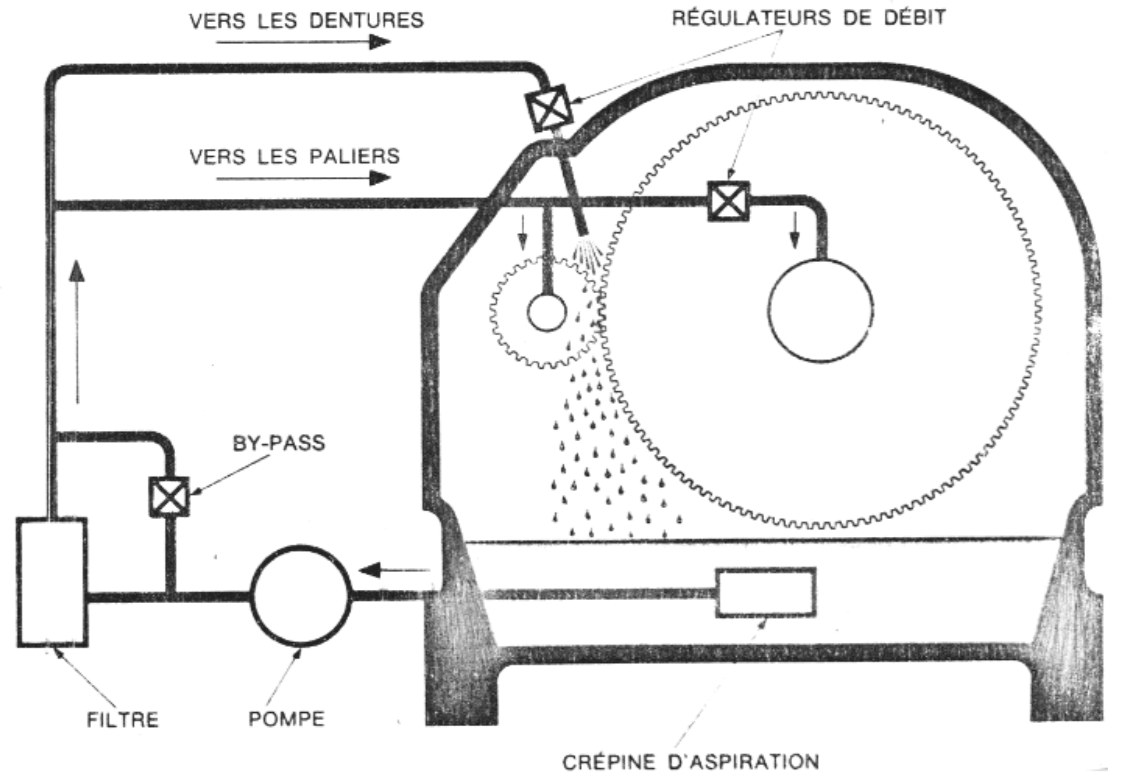
\includegraphics[scale=0.21]{ch1/15}
\end{wrapfigure}	
\noindent Ce mécanisme est utilisé pour de grosses puissances qui nécéssitent une lubrification dès le démarrage ainsi qu'un refroidissement important. Pour finir, dans le pire des cas, une lubrification par \textbf{graisse} peut protéger les pièces contre la corrosion, mais c'est sale. Notons que des pièces en \textbf{plastiques} sont également utilisées en raison de leur capacité auto-lubrifiante.
	
\section{Les engrenages cylindriques droits}
\subsection{Introduction}
Niveau, therminologie, on appellera \textbf{pignon} la roue menante et \textbf{engrenage} la roue menée. \\
Précisons qu'il existe deux normes : la norme \textbf{nord-américaine AGMA} (American Gear Manufacturers Association) et la norme \textbf{européenne}. 
	
\subsection{Géométrie des engrenages}
\subsubsection{Théorème du rapport de vitesses constantes}
\theor{\textsc{Théorème du rapport de vitesses constantes}\\
	\begin{wrapfigure}[6]{r}{4.5cm}
		\vspace{-10mm}
		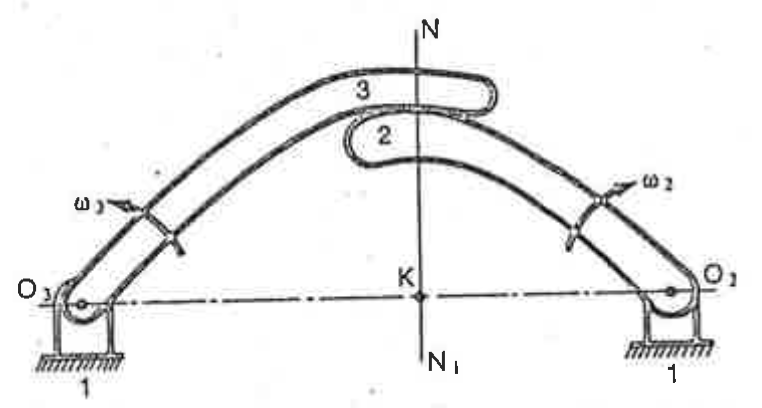
\includegraphics[scale=0.35]{ch1/16}
	\end{wrapfigure}	
	Pour une paire de surfaces courbes en contact, les vitesses angulaires sont inversément proportionnelles aux longueurs $0_2K$ et $O_3K$, où le point $K$ représente le point d'intersection de la normale commune avec la ligne des centres $O_2O_3$. On peut donc écrire 
	\begin{equation}
		\frac{\omega _2}{\omega _3} = \frac{O_3K}{O_2K}
	\end{equation}	}
\ \\
Ce théorème nous indique donc que pour avoir un rapport de vitesses contant, la normale commune doit intercepter la droite des centres en un point $K$ \textbf{fixe}. \\
Il existe deux théories qui mènent à la normalisation : la \textbf{développante de cercle} et la \textbf{cycloïde}. Nous n'allons nous interesser qu'à la développante.
	
\newpage	
	
\subsubsection{Illustration de la génération d'une développante de cercle}
\begin{wrapfigure}[12]{l}{4cm}
	\vspace{-5mm}
	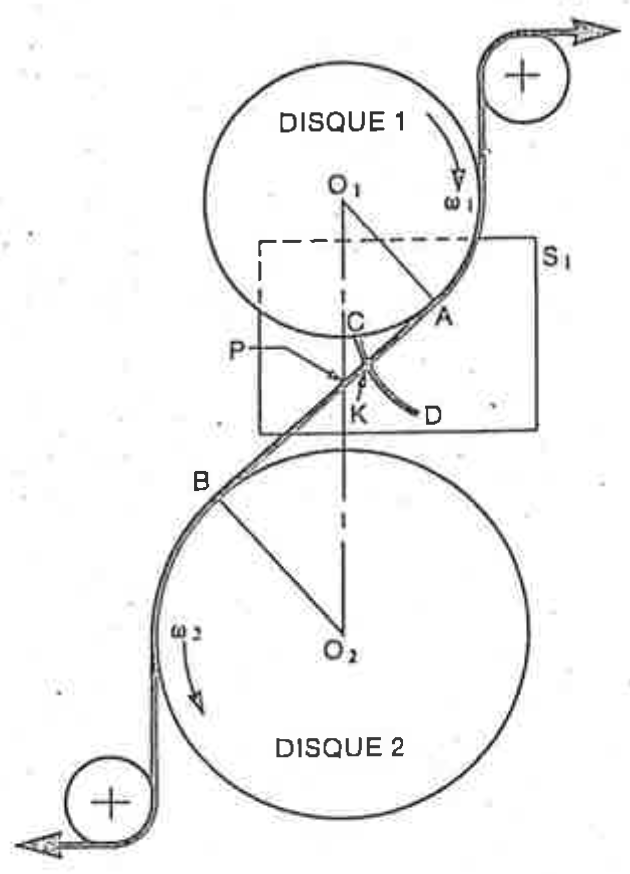
\includegraphics[scale=0.35]{ch1/17}
\end{wrapfigure}	
Nous avons vu une première méthode à la \autoref{subsec:1.2.2}. En voici une autre. Soient 2 disques, un pignon (petit) et un engrenage (grand) de centre fixe $O_1$ et $O_2$ et de rayon respectif $O_1A$ et $O_2B$. Ceux-ci sont entraîné par une corde sans glissement (supposition). Les points $A$ et $B$ correspondent alors aux points de tangence des disques et la corde. En traçant la ligne des centres, on coupe la ligne $AB$ au point $P$ qui est appelé \textbf{point primitif}. On a alors la relation 
\begin{equation}
	\frac{\omega _1}{\omega _2} = \frac{O_2B}{O_1A} = \frac{O_1P}{O_2P}
\end{equation}
Fixons à présent une plaque $S_1$ sur la roue menante et une pointe traçante au point $K$. Le point $C$ est obtenu lorsque $A$ et $K$ se superposent. De là, en déroulant la corde vers la gauche, on trace la courbe $CD$. La droite $AB$ est toujours perpendiculaire au profil $CD$ et le rayon de courbure est donné par la longueur $KA$.	\\
	
\begin{wrapfigure}[12]{r}{2.5cm}
	\vspace{-5mm}
	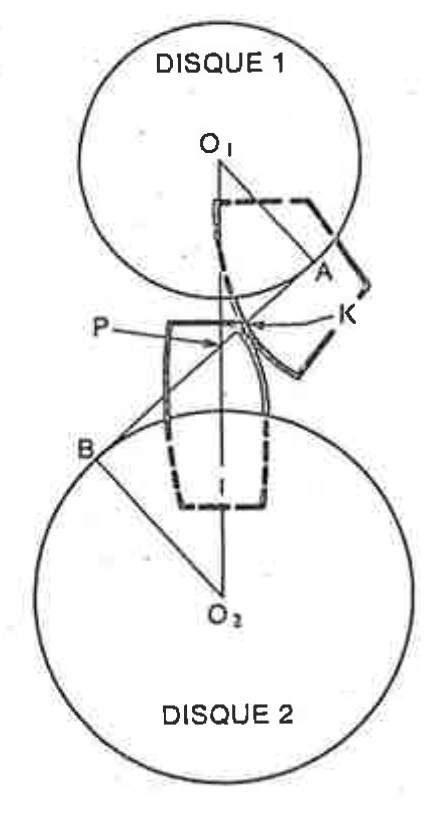
\includegraphics[scale=0.35]{ch1/18}
\end{wrapfigure}	
Faisons la même chose avec l'engrenage et découpons les plaques pour bien apercevoir le contact au point $K$ entre les courbes $CKD$ et $EKF$. La droite $AB$ est donc toujours perpendiculaire aux deux profils et coupe toujours la ligne des centres au point $P$. Tous les points de contact se trouvent sur cette \textbf{ligne de contact}. Le théorème étant satisfait, la vitesse d'engrenement est constant. \\
Les cercles de centre $O_1$ et $O_2$ passant par le point $P$ sont appelés \textbf{cercles primitifs}, alors que ceux de rayon $O_1A$ et $O_2B$ sont les \textbf{cercles de base}. L'angle $\phi$ entre la tangente commune $AB$ et la perpendiculaire à la ligne des centre s'appelle l'\textbf{angle de pression}.
	
\subsection{Propriété de la développante de cercle}
On va enfin pouvoir donner une relation mathématique pour l'angle de la développante, la fonction développante et l'épaisseur de la dent. 
	
\subsubsection{Angle de la développante}
\begin{wrapfigure}[12]{l}{5.5cm}
	\vspace{-5mm}
	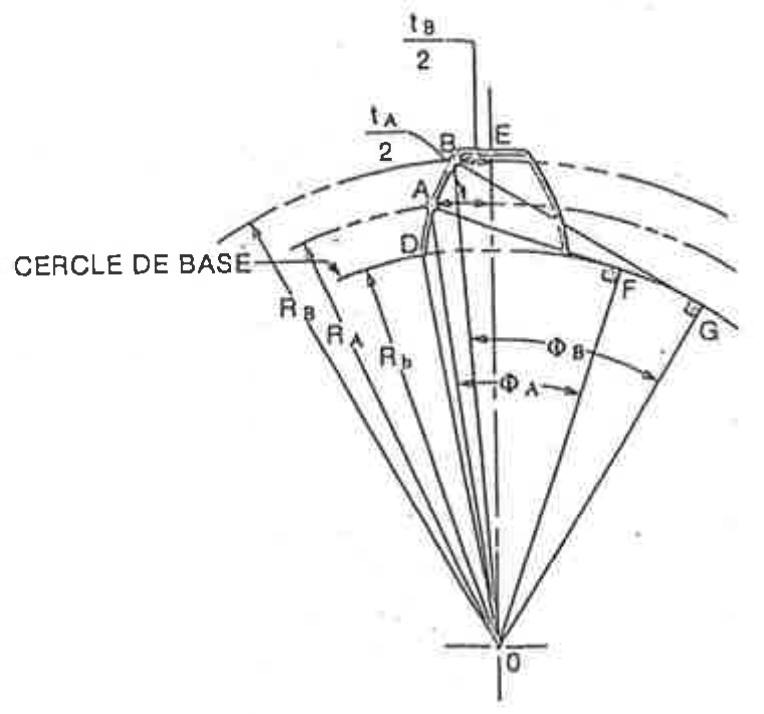
\includegraphics[scale=0.4]{ch1/19}
\end{wrapfigure}
Sur la figure ci-contre est représenté le cercle de base de rayon $R_b$ et une développante de cercle $DAB$. $F$ et $G$ sont les points de tangence des tangentes au cercle passant respectivement par $A$ et $B$. On définit alors les \textbf{angles de développante} $\phi _A$ et $\phi _B$ et les triangles rectangles $AOF$ et $BOG$ qui nous permettent d'écrire
\begin{equation}
	R_b = R_A \cos \phi _A \qquad and \qquad R_b = R_B \cos \phi _B
\end{equation}
donc 
\begin{equation}
	\cos \phi _B = \frac{R_A}{R_B} \cos \phi _A
\end{equation}
Cette relation nous permet de déterminer l'angle de développante pour tout point du profil, au départ d'une connu pour un rayon donné. Prenons maintenant $A$ sur le cercle de base tel que $R_A = R_b$ et $\phi _A = 0 \rightarrow \cos \phi _A = 1$. Si $B$ est sur le cercle primitif et que $R_B = R$, $\phi _B = \phi$, alors 
	
\begin{equation}
	R_b = R \cos \phi \qquad \mbox{(relation entre cercle de base et cercle primitif)}
\end{equation}	 
	
\subsubsection{Fonction développante}
Sur la figure ci-dessus, on peut exprimer l'angle $DOG$ comme
\begin{equation}
	\angle DOG = \frac{\mbox{arc } DG}{OG}
\end{equation}
Grâce à une propriété des développante de cercle, l'arc $DG = BG$ (on déballe la corde). Sachant que $\tan \phi _B = \frac{BG}{OG}$, on peut calculer l'angle $DOB$ 
\begin{equation}
	\angle DOB = \angle DOG - \phi _B \qquad \Leftrightarrow \qquad inv \, \phi _B= \tan \phi _B - \phi _B
	\label{equation:1.7}
\end{equation}
Cette dernière expression se nomme \textbf{fonction développante ou involute}. Ce développement est aussi valable pour $\phi _A$.
	
\subsubsection{Epaisseur de la dent}
Toujours basé sur la même figure, soient $t_A$ et $t_B$ l'épaisseur de la dent au point $B$ et $A$ et le rayon $OE = R_B$ passant par le centre de la dent. On peut écrire 
\begin{equation}
	\angle DOE = \angle DOB + \frac{1}{2}\frac{t_B}{R_B}
\end{equation}
En utilisant l'équation \autoref{equation:1.7}, on trouve (de même pour le point $A$)
\begin{equation}
	\angle DOE = inv \, \phi_B + \frac{1}{2}\frac{t_B}{R_B} \qquad et \qquad 		\angle DOE = inv \, \phi_A + \frac{1}{2}\frac{t_A}{R_A}
\end{equation}
L'égalisation des deux équations nous donne la relation finale
\begin{equation}
	t_B = 2R_B \left[ \frac{t_A}{2R_A} + (inv \, \phi _A - inv \, \phi _B) \right]
	\label{eq:1.10}
\end{equation}
qui, de nouveau, nous permet de connaître l'épaisseur en nimporte quel rayon à condition de connaître l'épaisseur et l'$inv \, \phi _A$ en un autre rayon.
	
\subsection{Définitions et normalisation}
Un système normalisé de dentures spécifie des relations afin de permettre l'interchangeabilité des engrenages ayant un même pas et un même angle de pression. C'est ici que les nord-Américains et les Européens divergent et il n'est malheureusement pas possible d'interchanger les engrenages d'un système à l'autre. 

\subsubsection{Approche nord-américaine}
Introduisons tout d'abord le \textbf{pas diamétrale} 
\begin{equation}
	P = \frac{N}{D_p}
\end{equation}
où $N$ est le nombre de dentures et $D_p$ le diamètre du cercle primitif (en pouces). Dans cette approche, les unités sont des $1/po$ (1/pouces).
		
\subsubsection{Approche européenne}
Ces unités étant bizarres, les Européens préfèrent utiliser le \textbf{module}
\begin{equation}
	M_o = \frac{25.4}{P}
\end{equation}
		
\subsubsection{Pas diamétrale}
Le pas diamétrale a été définie ci-dessus. Il représente la grosseur de la dent. Plus il est grand, plus la dent est petite. Afin de limiter le nombre de $P$ différent, il existe des valeurs normalisées. Avoir le même pas diamétrale est une condition nécéssaire d'engrenement. 
		
\subsubsection{L'angle de pression}		
L'angle de pression $\phi$ est l'angle de développante au rayon promitif de l'engrenage. Normalisés également, ils sont au nombre de 3 : $14.5\degres$, $20\degres$ et $25\degres$. Il faut savoir que l'épaisseur de la dent en sa base augmente avec l'angle en raison du support de plus grande contrainte. 
		
\subsubsection{Le pas primitif}
Noté $p$, c'est la distance entre 2 dents consécutives mesuré sur le cercle primitif (à ne pas confonre avec $p_b$ qui est pour le cercle de base). 
\begin{equation}
	p = 2\pi \frac{R}{N} = \pi \frac{D}{N} = \frac{\pi}{P} \qquad et \qquad p_b = 2\pi \frac{R_b}{N}
	\label{eq:1.13}
\end{equation}
		
\subsubsection{Saillie et creux}
\begin{wrapfigure}[7]{l}{5.5cm}
	\vspace{-5mm}
	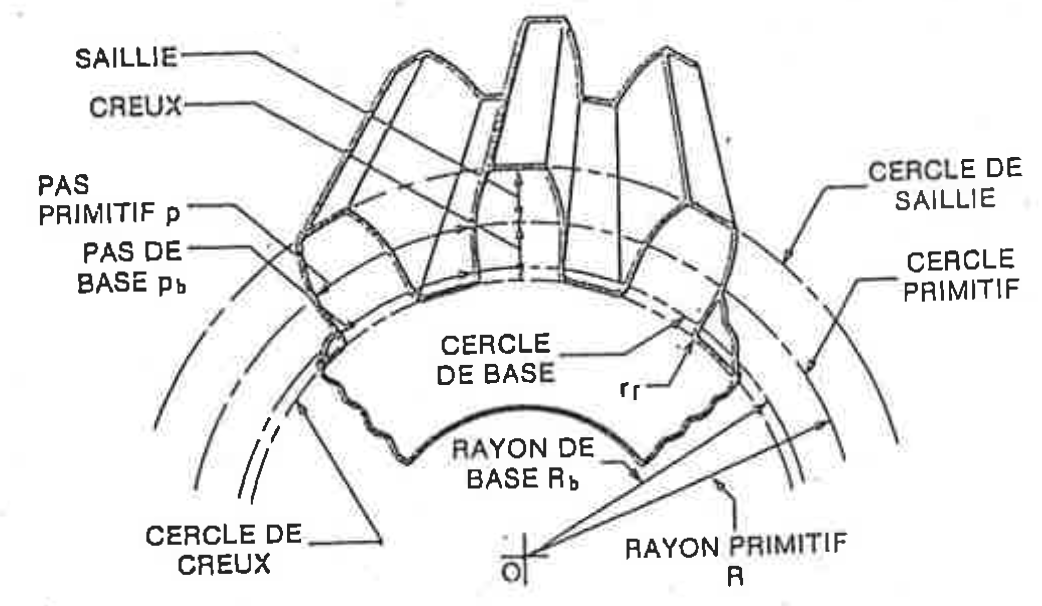
\includegraphics[scale=0.3]{ch1/20}
\end{wrapfigure}		
La saillie est la distance radiale du sommet de la dent au cercle primitif. Le creux est la distance de ce cercle à la racine de la dent. Les cercles passant du sommet et de la racine sont appelés le cercle de \textbf{saillie} et de \textbf{creux}. C'est à cause du creux qu'aparaissent les phénomènes d'\textbf{interférences}. \\
La somme de la saillie et du creux est la \textbf{hauteur} (normalisée). \\
La ligne de contact est celle selon laquelle le point de contact se déplace, c'est la tangente aux cercles de base. 
		
\begin{wrapfigure}[4]{r}{4cm}
	\vspace{-5mm}
	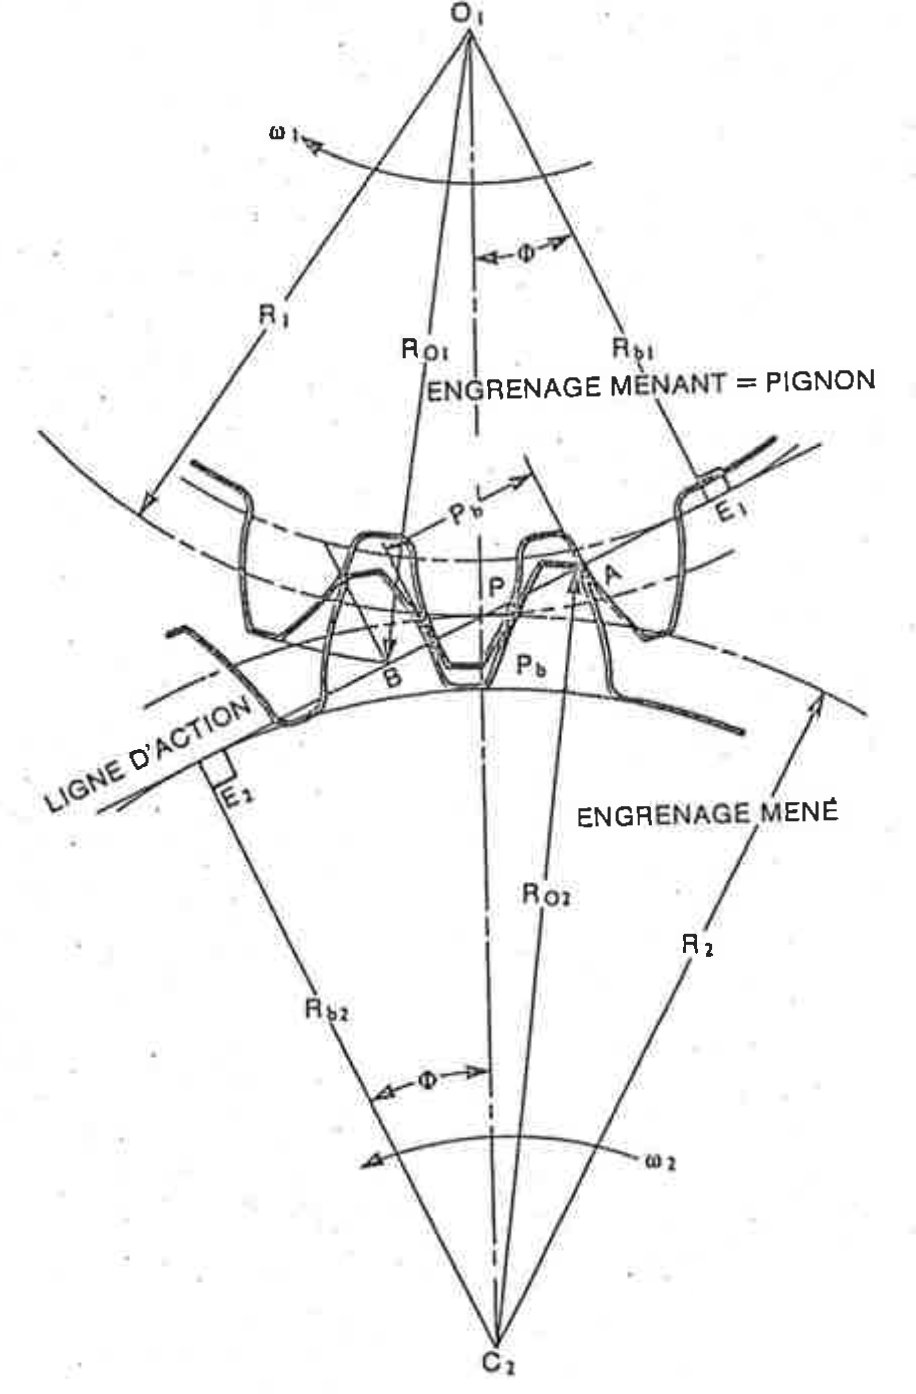
\includegraphics[scale=0.25]{ch1/21}
\end{wrapfigure}				 
\subsubsection{Longueur d'action}
Le point $A$ et $B$ correspondent respectivement au point d'entrée et de sortie de contact, où les cercles de saillie coupent la ligne d'action. La portion de la ligne d'action délimitée par $AB$ s'appelle la \textbf{longueur d'action}.
		
\subsubsection{Distance des centres C}
C'est la distance totale entre les centres des deux engrenages qu'on peut calculer selon
\begin{equation}
	C = R_1 + R_2 = \frac{N_1 + N_2}{2P}
\end{equation}
		
\subsubsection{Jeu radial}
Il a dit qu'on y reviendra la semaine prochaine. 
		
		
\subsubsection{Crémaillère}
On a vu ce cas particulier plus haut. On ne parle plus ici de cercle primitif mais bien de \textbf{ligne primitive} en raison d'un diamètre infini. 
		
\subsection{Etude du mouvement du point de contact}		
\begin{wrapfigure}[7]{l}{4.5cm}
	\vspace{-5mm}
	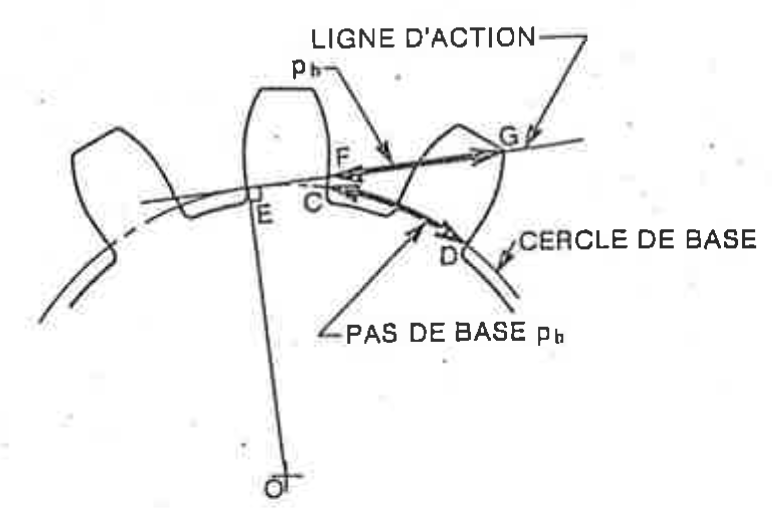
\includegraphics[scale=0.35]{ch1/22}
\end{wrapfigure}				 
Les caractéristiques énoncées pour la longueur d'action sont importantes. Rappelons que la ligne d'action est simultanément la tangente aux deux cercles et au point de contact. \\
La figure ci-contre nous montre que le pas de base peut aussi être calculer d'une autre manière.\\
	
\begin{proof} \ \\
	Remarquons que les profils de développante de cercle nous permettent d'égaliser les longueurs 
	
	\begin{equation}
		\mbox{arc } EC = EF \qquad et \qquad \mbox{arc } ED = EG
	\end{equation}				
			
	En soustrayant les deux arcs pour avoir l'arc $CD$ on a 
	\begin{equation}
		\mbox{arc } CD = p_b = FG
	\end{equation}				
\end{proof}
	
Par ailleurs, il faut s'assurer qu'une paire au moins de dents est en contact. Pour cela on a définit le \textbf{rapport de conduite}
\begin{equation}
	m = \frac{\mbox{longueur d'action}}{\mbox{pas de base}} = \frac{AB}{p_b}
\end{equation}
On calcule la longueur d'action de la manière suivante
\begin{equation}
	AB = E_1B + E_2A -E_1E_2
\end{equation}
Par trigonométrie (triangle rectangle) on a, avec $R_o$ désignant les rayons de saillie, les relations
\begin{equation}
	E_1B = \sqrt{R_{o1}^2-R_{b1}^2} \qquad E_1A = \sqrt{R_{o2}^2-R_{b2}^2} \qquad E_1E_2 = E_1P + PE_2 = (R_1 + R_2) \sin \phi
\end{equation}
En mettant tout ça dans notre équation de base, on a
\begin{equation}
	AB = \sqrt{R_{o1}^2-R_{b1}^2} + \sqrt{R_{o2}^2-R_{b2}^2} - (R_1 + R_2) \sin \phi
\end{equation}
Le pas de base $p_B$ de l'équation \autoref{eq:1.13} finalise l'expression de $m$
\begin{equation}
	m = \frac{\sqrt{R_{o1}^2-R_{b1}^2} + \sqrt{R_{o2}^2-R_{b2}^2} - (R_1 + R_2) \sin \phi}{2\pi R_b/N}
\end{equation}
Pour avoir au moins une pair de dents en contact, il faut que $m$ soit supérieur à l'unité. Les manufacturiers conseillent $m = 1.4$ minimum. Si on a par exemple $1.6$, alors 2 dents sont en contact $60 \%$ du temps.
		
\subsection{Interchangeabilité des engrenages}
Comment est-ce qu'on peut faire fonctionner les engrenages ? 
\begin{enumerate}
	\item Il faut absolument que les engrenages aient une normale commune. Pour ça, il faut une ligne d'action commune et donc le même angle de pression.
	      		
	\item Il faut que les deux dents puissent s'engrener, donc le même diamètre et donc le même module ou pas diamétrale. \\
\end{enumerate}		 

On pourrait croire que ça suffit, sauf que ça ne marche pas toujours. Les 2 conditions sont nécessaires mais pas suffisantes. La $3\up{ème}$ à vérifier est que $A$ et $B$ soit à l'intérieur de la longueur de contact maximale $E_1E_2$. Si ce n'est pas le cas, on n'est pas sur la ligne de contact commune quand les deux dents entrent en contact. \\
On appelle alors \textbf{phénomène d'interférence} le cas où, si le pignon est trop petit par rapport à l'engrenage, la tête de la dent de l'engrenage ne peut s'engager physiquement dans le creux du pignon et va causer de l'érosion à la racine de la dent du pignon.\\
Ceci est dû au fait que le cercle de creux est plus petit que le cercle de base et le profil de développante ne commence qu'au cercle de base. Par conséquent, la condition de rapport de vitesse constante n'est plus respectée. En conclusion, on fera attention à ce que 
\begin{equation}
	AP < E_1P \qquad et \qquad PB < E_2P
\end{equation}
On se pose alors la question de si un engrenage comporte un certain nombre de dents, quel doit être le nombre de dents sur l'autre engrenage pour éviter l'interférence ? On sait premièrement que 
\begin{equation}
	E_1P-AP \geq 0
	\label{eq:1.23}
\end{equation}

	\begin{wrapfigure}[7]{l}{5.5cm}
	\vspace{-10mm}
	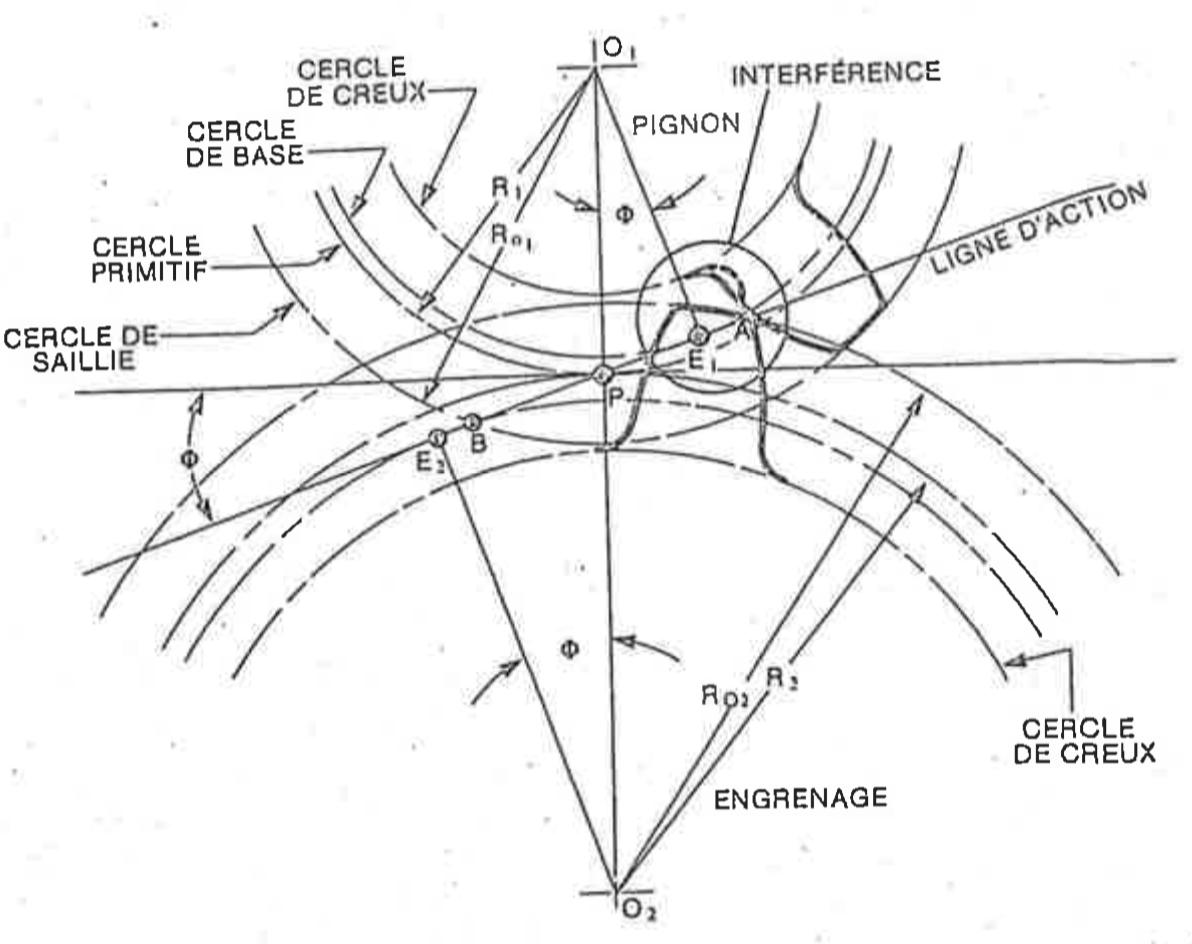
\includegraphics[scale=0.25]{ch1/23}
	\end{wrapfigure}				 
	Utilisons les règles géométriques pour exprimer ces deux longueurs selon le nombre de dents (v. figure ci-contre), sachant que $N_1<N_2$
	\begin{equation}
		E_1P = R_1\sin \phi = \frac{N_1}{2P}\sin \phi 
		\label{eq:1.24}
	\end{equation}
	Par ailleurs $AP = E_2A - E_2P$ avec 
	\begin{equation}
		E_2A = \sqrt{R_{02}^2-R_{b2}^2} = \sqrt{R_{02}^2-R_{2}^2\cos ^2 \phi}
	\end{equation}
	Pour les engrenages normalisés, on peut écrire la relation $R_0 = R+a$ où $a=\frac{k}{P}$. L'équation précédente devient
	\begin{equation}
	E_2A= \sqrt{\left( R_2+\frac{k}{P} \right)^2-R_{2}^2\cos ^2 \phi} = \sqrt{\left( \frac{N_2}{2P}+\frac{2k}{2P} \right)^2-\left( \frac{N_2}{2P}\cos \phi \right) ^2}
	\end{equation}
	Dernièrement, comme l'équation \autoref{eq:1.24}, $E_2P = \frac{N_2}{2P}\sin \phi$. En réécrivant l'équation \autoref{eq:1.23}, on a 
	\begin{equation}
		\frac{N_1}{2P}\sin \phi - \frac{1}{2P}\left[ \sqrt{(N_2 + 2k)^2 - (N_2 \cos \phi )^2} - N_2 \sin \phi \right] \geq 0
	\end{equation}
	Les dénominateurs sont positifs d'après la définition de P, on peut donc se concentrer sur le numérateur. Si on met en évidence le $\sin$ dans un membre et qu'on passe la racine dans l'autre membre, après élévation au carré on a 
	\begin{equation}
		(N_1+N_2)^2\sin ^2 \phi - (N_2+2k)^2 + (N_2\cos \phi)^2 \geq 0
	\end{equation}
	On obtient la fonction $g(N_1,N_2)$ qui permet d'éviter l'interférence en développant les carrés et en remarquant que $N_2$ s'annule
	\begin{equation}
		g(N_1,N_2) = (N_1^2 + 2N_1N_2)\sin ^2 \phi - 4kN_2 - 4k^2  \geq 0
		\label{eq:1.29}
	\end{equation}
	
	\subsubsection{Engagement pignon-crémaillère}
		\begin{wrapfigure}[8]{l}{4cm}
		\vspace{-5mm}
		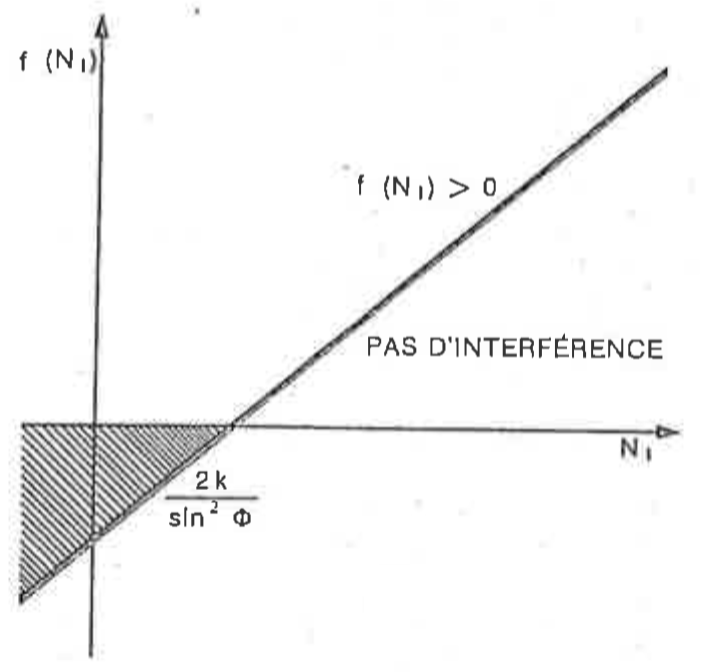
\includegraphics[scale=0.3]{ch1/24}
		\end{wrapfigure}				 
		Dans ce cas, $R_2= \infty$ et pose problème avec notre équation \autoref{eq:1.29}. On la divise alors par $N_2$ et on fait tendre $N_2$ vers l'infini pour obtenir
		\begin{equation}
			f(N_1) = 2N_1\sin ^2\phi - 4k \geq 0 
		\end{equation}
		Le zéro de la fonction est $N_1 = \frac{2k}{\sin \phi}$. Etudions l'allure de la fonction $f(N_1)$. La dérivée première par rapport à $N_1$ est une constante et le zéro représente le plus petit nombre de dents sur le pignon pour éviter l'interférence. \\

		\begin{wrapfigure}[3]{r}{3.7cm}
		\vspace{-5mm}
		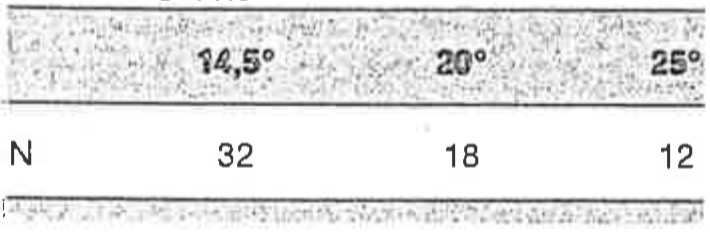
\includegraphics[scale=0.3]{ch1/25}
		\end{wrapfigure}		
		Pour un engrenage normalisé $k = 1$. Dans ce cas, le nombre de dents n'est fonction que de l'angle de pression. Le tableau ci-contre reprend les différentes valeurs de $N_1$ pour 3 angles selon l'équation trouvée. Physiquement, si un pignon de $N$ dents s'engage dans une crémaillère, il fonctionnera sans interférence avec un engrenage de même saillie dont le nombre de dents est compris entre l'infini et $N$. Par exemple pour $\phi = 20\degres$, un pignon de 18 dents nécessite un engrenage de minimum 18 dents. 
		
	\subsubsection{Engagement de deux engrenages identiques}
		\begin{wrapfigure}[8]{l}{4cm}
		\vspace{-5mm}
		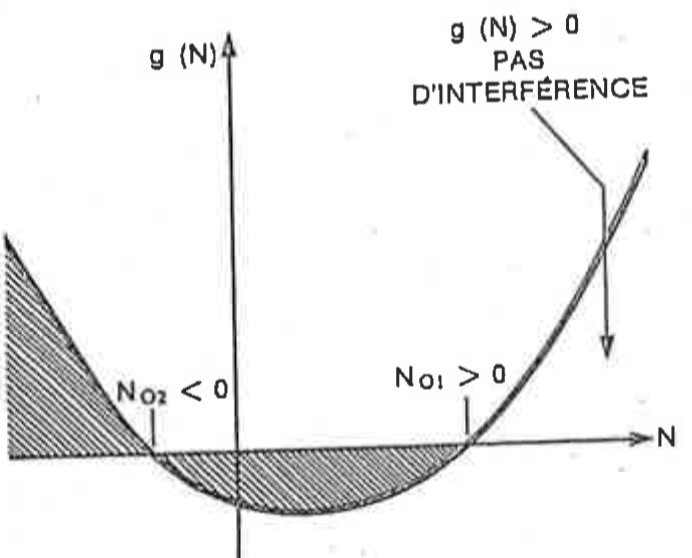
\includegraphics[scale=0.3]{ch1/26}
		\end{wrapfigure}				
		Dans le cas où $N_1=N_2=N$, l'équation \autoref{eq:1.29} devient 
		\begin{equation}
			g(N) = 3N^2\sin ^2 \phi - 4kN - 4k^2 \geq 0
		\end{equation}
		où les zéros sont donnés par 
		\begin{equation}
			N_{1,2} = \frac{2k}{3\sin ^2 \phi} (1 \pm \sqrt{3 \sin ^2 \phi})
		\end{equation}
		La dérivée première peut être positive, négative ou nulle et la dérivée seconde est toujours positive. On peut voir sur l'image que le zéro positif représente le minimum comme précédemment. 

		\begin{wrapfigure}[3]{r}{4cm}
		\vspace{-5mm}
		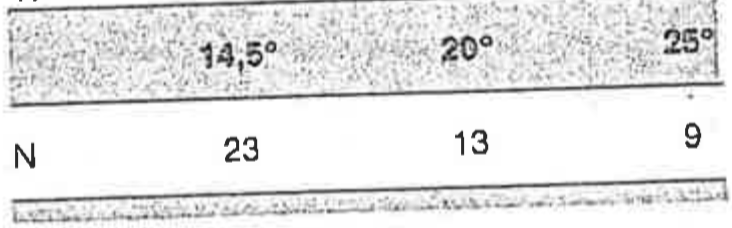
\includegraphics[scale=0.3]{ch1/28}
		\end{wrapfigure}				
		Cette valeur pour un angle de pression de $20\degres$ est de 13 dents. \\
		On a trouver une valeur au dessus de laquelle on a jamais interférence avec le premier cas et une valeur en dessous de laquelle on a toujours interférence avec le deuxième. Il reste le cas entre ces deux valeurs. 
		
		\subsubsection{Engagement de deux engrenages lorsque N1 est connu}
		\begin{wrapfigure}[8]{l}{3.8cm}
		\vspace{-5mm}
		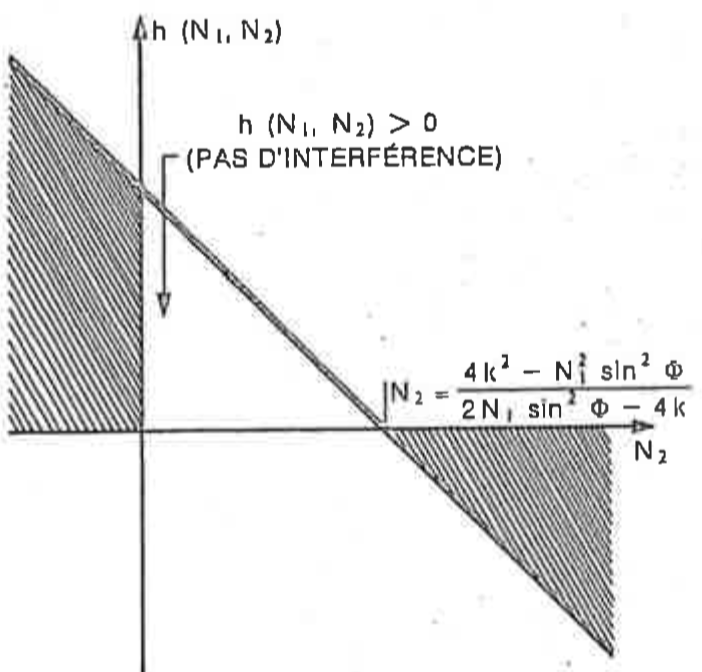
\includegraphics[scale=0.3]{ch1/27}
		\end{wrapfigure}		
		Supposons que $N_1$ est connu, plus petit que $N_2$ et est situé entre les valeurs déterminées dans les deux cas précédents. On reprend alors l'équation \autoref{eq:1.29} dont le zéro est 
			\begin{equation}
				N_2 = \frac{4k^2 - N_1 ^2 \sin ^2 \phi}{2 N_1 \sin ^2 \phi - 4k}
				\label{eq:1.33}
			\end{equation}
			Si nous étudions l'allure de la fonction, on voit que la dérivée première est constante et négative pour toute valeur plus petite que le nombre minimal (v. tableau des 2 autres cas). On peut voir sur la figure que le zéro représente le plus grand nombre pour éviter l'interférence. 
			
		\subsubsection{Engagement de deux engrenages lorsque N2 est connu}
			\begin{wrapfigure}[5]{l}{4cm}
			\vspace{-5mm}
			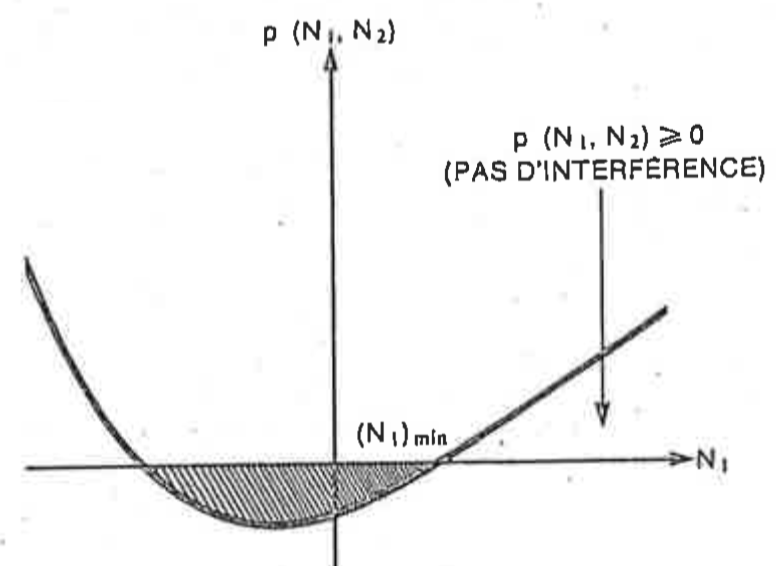
\includegraphics[scale=0.3]{ch1/29}
			\end{wrapfigure}					
			Toujours pour $N_1<N_2$, on reprend l'équation \autoref{eq:1.29} et ses zéros, exprimés cette fois en tant que $N_1$ sont
			\begin{equation}
				(N_1)_i = - N_2 \pm \sqrt{N_2^2 + \frac{4}{\sin ^2 \phi}(kN_2 +k^2)}
				\label{eq:1.34}
			\end{equation}
			Si nous étudions l'allure de la fonction $p(N_1,N_2)$, la dérivée première par rapport à $N_1$ et la dérivée seconde sont toutes les deux positives. On voit que la racine positive représente le plus petit nombre de dents avant interférence. \\
			
			En résumé, il faut distinguer les cas pignon-crémaillère et engrenages identiques. Sinon, on doit calculer le \textbf{nombre minimum de dents} avec lequel il peut s'engager en utilisant l'équation \autoref{eq:1.34} et le \textbf{nombre maximum de  dents} avec lequel il peut s'engager en utilisant \autoref{eq:1.33}.
			
\section{Jeu entre les deux engrenages}
	\subsection{Distance entre les centres C}
		La distance entre les cercles est exprimé selon 
		\begin{equation}
			C = \frac{N_1 + N_2}{2P}
		\end{equation}
		et le rapport des vitesses est exprimé selon 
		\begin{equation}
			\frac{\omega _1}{\omega _2} = \frac{N_2}{N_1}
		\end{equation}
		On voit qu'il n'y a pas de lien entre ces deux équations et il peut y avoir incompatibilité. Si en pratique, la distance entre les centres n'est pas la même que celle donnée par l'équation ci-dessus, il y aura un jeu radial plus important que celui prévu et le jeu au cercle primitif ne sera pas nul. Cette condition va se retrouver dans tous les montages à cause des tolérances permises. \\
		
		\begin{wrapfigure}[8]{r}{6.5cm}
		\vspace{-5mm}
		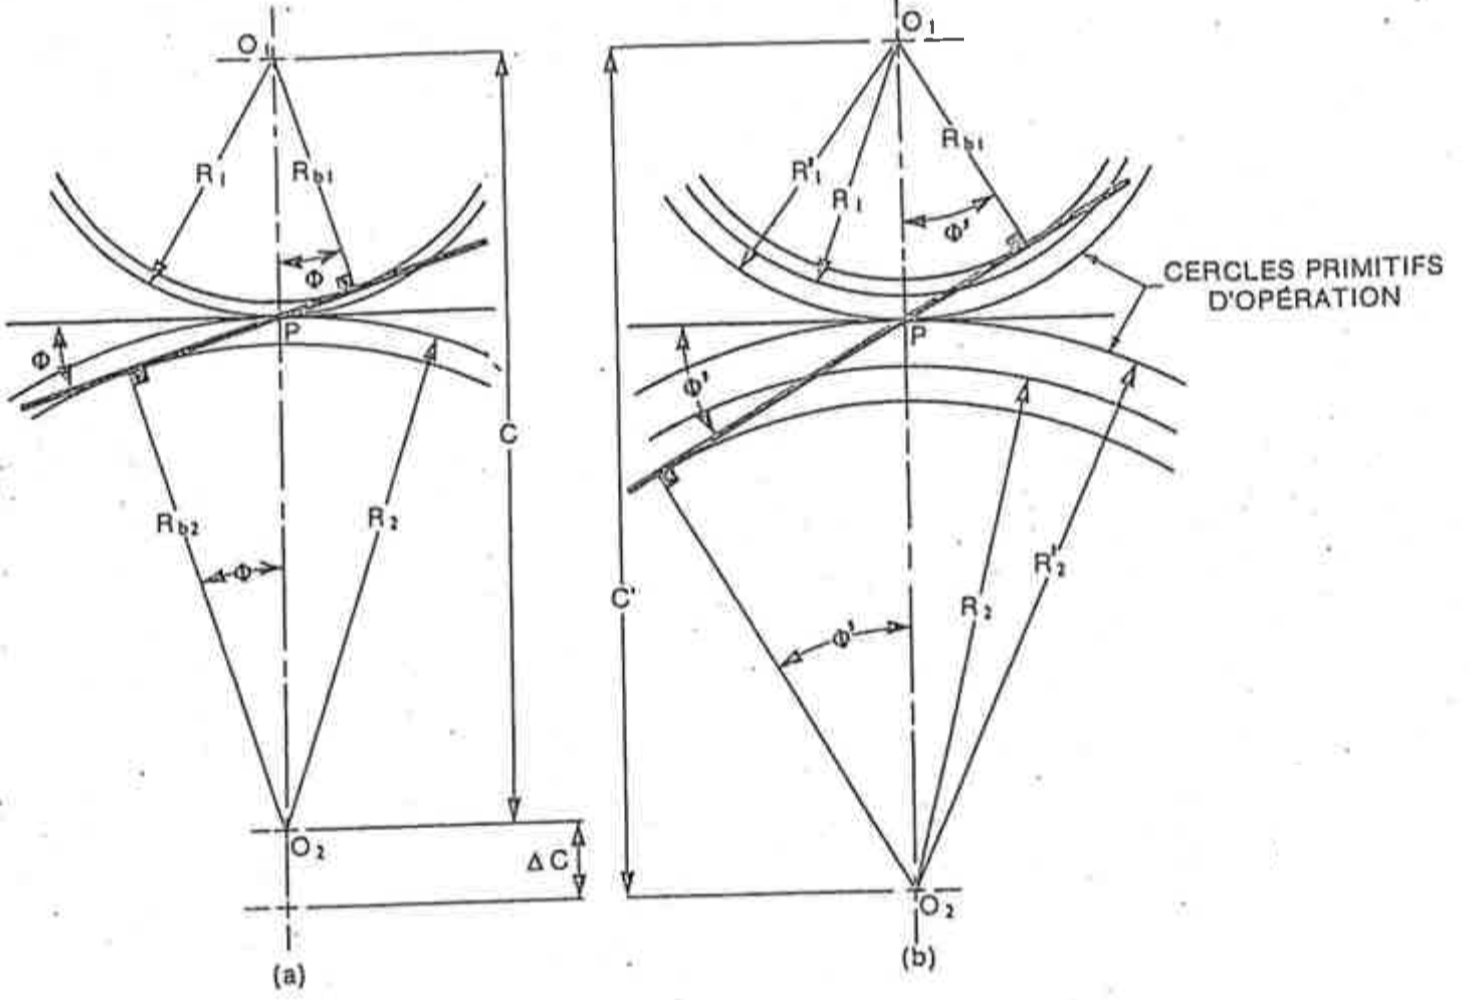
\includegraphics[scale=0.25]{ch1/30}
		\end{wrapfigure}			
		Si la distance entre les centres est augmentée de $\Delta C$, ona $C' = C + \Delta C$. Comme l'illustre le montage ci-contre, les cercles primitifs $R'_1$ et $R'_2$ ne coïncident plus avec ceux de départ, contrairement aux cercles de base et au rapport des vitesses. L'angle de pression devient $\phi '$. Donc 
		\begin{equation}
		\frac{\omega _1}{\omega _2} = \frac{N_2}{N_1} = \frac{R'_2}{R'_1} \qquad C' = R'_1 + R'_1 \frac{N_2}{N_1}
		\end{equation}
		D'où 
		\begin{equation}
			R'_1 = C' \left( \frac{N_1}{N_1+N_2} \right) \qquad et \qquad R'_2 = C' \left( \frac{N_2}{N_1+N_2} \right)
		\end{equation}
		D'autre part 
		\begin{equation}
			R'_1 = \frac{R_{b1}}{\cos \phi '} \qquad 	R'_2 = \frac{R_{b2}}{\cos \phi '} \qquad et \qquad R_{b1} = R_1 \cos \phi \qquad R_{b2} = R_2 \cos \phi
		\end{equation}
		nous donnent la relation pour $C'$ et $\phi '$
		\begin{equation}
			C' = \frac{R'_1+R'_2}{\cos \phi '} = \frac{C \cos \phi}{\cos \phi '} \qquad \Rightarrow \qquad \phi ' = \arccos \left( \frac{C}{C'} \cos \phi \right)
		\end{equation}
		
	\subsection{Jeu au cercle primitif}
		A cause de l'augmentation de la distance entre les centres, les cercles primitifs ne coïncident plus. Pour un jeu $B$, le pas circulaire mesuré sur le cercle primitif d'opération sera exprimé comme
		\begin{equation}
			t'_1 + t'_2 + B = \frac{2\pi R'_1}{N_1} = \frac{2\pi R'_2}{N_2}
		\end{equation}
		Si on remonte bien plus haut, selon l'équation \autoref{eq:1.10} on peut écrire
		\begin{equation}
			t'_1 = 2R'_1\left( \frac{t_1}{2R_1} + inv \phi - inv \phi ' \right) = \frac{R'_1}{R_1} t_1 - 2R'_1(inv\phi ' - inv \phi)
		\end{equation}
		De même $t'_2 = \frac{R'_2}{R_2} t_2 - 2R'_2(inv\phi ' - inv \phi)$. 